% Options for packages loaded elsewhere
\PassOptionsToPackage{unicode}{hyperref}
\PassOptionsToPackage{hyphens}{url}
%
\documentclass[
]{article}
\usepackage{amsmath,amssymb}
\usepackage{lmodern}
\usepackage{ifxetex,ifluatex}
\ifnum 0\ifxetex 1\fi\ifluatex 1\fi=0 % if pdftex
  \usepackage[T1]{fontenc}
  \usepackage[utf8]{inputenc}
  \usepackage{textcomp} % provide euro and other symbols
\else % if luatex or xetex
  \usepackage{unicode-math}
  \defaultfontfeatures{Scale=MatchLowercase}
  \defaultfontfeatures[\rmfamily]{Ligatures=TeX,Scale=1}
\fi
% Use upquote if available, for straight quotes in verbatim environments
\IfFileExists{upquote.sty}{\usepackage{upquote}}{}
\IfFileExists{microtype.sty}{% use microtype if available
  \usepackage[]{microtype}
  \UseMicrotypeSet[protrusion]{basicmath} % disable protrusion for tt fonts
}{}
\makeatletter
\@ifundefined{KOMAClassName}{% if non-KOMA class
  \IfFileExists{parskip.sty}{%
    \usepackage{parskip}
  }{% else
    \setlength{\parindent}{0pt}
    \setlength{\parskip}{6pt plus 2pt minus 1pt}}
}{% if KOMA class
  \KOMAoptions{parskip=half}}
\makeatother
\usepackage{xcolor}
\IfFileExists{xurl.sty}{\usepackage{xurl}}{} % add URL line breaks if available
\IfFileExists{bookmark.sty}{\usepackage{bookmark}}{\usepackage{hyperref}}
\hypersetup{
  pdftitle={homework\_02},
  pdfauthor={Esteban Jorquera; Marlon Aldair; Diego},
  hidelinks,
  pdfcreator={LaTeX via pandoc}}
\urlstyle{same} % disable monospaced font for URLs
\usepackage[margin=1in]{geometry}
\usepackage{color}
\usepackage{fancyvrb}
\newcommand{\VerbBar}{|}
\newcommand{\VERB}{\Verb[commandchars=\\\{\}]}
\DefineVerbatimEnvironment{Highlighting}{Verbatim}{commandchars=\\\{\}}
% Add ',fontsize=\small' for more characters per line
\usepackage{framed}
\definecolor{shadecolor}{RGB}{248,248,248}
\newenvironment{Shaded}{\begin{snugshade}}{\end{snugshade}}
\newcommand{\AlertTok}[1]{\textcolor[rgb]{0.94,0.16,0.16}{#1}}
\newcommand{\AnnotationTok}[1]{\textcolor[rgb]{0.56,0.35,0.01}{\textbf{\textit{#1}}}}
\newcommand{\AttributeTok}[1]{\textcolor[rgb]{0.77,0.63,0.00}{#1}}
\newcommand{\BaseNTok}[1]{\textcolor[rgb]{0.00,0.00,0.81}{#1}}
\newcommand{\BuiltInTok}[1]{#1}
\newcommand{\CharTok}[1]{\textcolor[rgb]{0.31,0.60,0.02}{#1}}
\newcommand{\CommentTok}[1]{\textcolor[rgb]{0.56,0.35,0.01}{\textit{#1}}}
\newcommand{\CommentVarTok}[1]{\textcolor[rgb]{0.56,0.35,0.01}{\textbf{\textit{#1}}}}
\newcommand{\ConstantTok}[1]{\textcolor[rgb]{0.00,0.00,0.00}{#1}}
\newcommand{\ControlFlowTok}[1]{\textcolor[rgb]{0.13,0.29,0.53}{\textbf{#1}}}
\newcommand{\DataTypeTok}[1]{\textcolor[rgb]{0.13,0.29,0.53}{#1}}
\newcommand{\DecValTok}[1]{\textcolor[rgb]{0.00,0.00,0.81}{#1}}
\newcommand{\DocumentationTok}[1]{\textcolor[rgb]{0.56,0.35,0.01}{\textbf{\textit{#1}}}}
\newcommand{\ErrorTok}[1]{\textcolor[rgb]{0.64,0.00,0.00}{\textbf{#1}}}
\newcommand{\ExtensionTok}[1]{#1}
\newcommand{\FloatTok}[1]{\textcolor[rgb]{0.00,0.00,0.81}{#1}}
\newcommand{\FunctionTok}[1]{\textcolor[rgb]{0.00,0.00,0.00}{#1}}
\newcommand{\ImportTok}[1]{#1}
\newcommand{\InformationTok}[1]{\textcolor[rgb]{0.56,0.35,0.01}{\textbf{\textit{#1}}}}
\newcommand{\KeywordTok}[1]{\textcolor[rgb]{0.13,0.29,0.53}{\textbf{#1}}}
\newcommand{\NormalTok}[1]{#1}
\newcommand{\OperatorTok}[1]{\textcolor[rgb]{0.81,0.36,0.00}{\textbf{#1}}}
\newcommand{\OtherTok}[1]{\textcolor[rgb]{0.56,0.35,0.01}{#1}}
\newcommand{\PreprocessorTok}[1]{\textcolor[rgb]{0.56,0.35,0.01}{\textit{#1}}}
\newcommand{\RegionMarkerTok}[1]{#1}
\newcommand{\SpecialCharTok}[1]{\textcolor[rgb]{0.00,0.00,0.00}{#1}}
\newcommand{\SpecialStringTok}[1]{\textcolor[rgb]{0.31,0.60,0.02}{#1}}
\newcommand{\StringTok}[1]{\textcolor[rgb]{0.31,0.60,0.02}{#1}}
\newcommand{\VariableTok}[1]{\textcolor[rgb]{0.00,0.00,0.00}{#1}}
\newcommand{\VerbatimStringTok}[1]{\textcolor[rgb]{0.31,0.60,0.02}{#1}}
\newcommand{\WarningTok}[1]{\textcolor[rgb]{0.56,0.35,0.01}{\textbf{\textit{#1}}}}
\usepackage{longtable,booktabs,array}
\usepackage{calc} % for calculating minipage widths
% Correct order of tables after \paragraph or \subparagraph
\usepackage{etoolbox}
\makeatletter
\patchcmd\longtable{\par}{\if@noskipsec\mbox{}\fi\par}{}{}
\makeatother
% Allow footnotes in longtable head/foot
\IfFileExists{footnotehyper.sty}{\usepackage{footnotehyper}}{\usepackage{footnote}}
\makesavenoteenv{longtable}
\usepackage{graphicx}
\makeatletter
\def\maxwidth{\ifdim\Gin@nat@width>\linewidth\linewidth\else\Gin@nat@width\fi}
\def\maxheight{\ifdim\Gin@nat@height>\textheight\textheight\else\Gin@nat@height\fi}
\makeatother
% Scale images if necessary, so that they will not overflow the page
% margins by default, and it is still possible to overwrite the defaults
% using explicit options in \includegraphics[width, height, ...]{}
\setkeys{Gin}{width=\maxwidth,height=\maxheight,keepaspectratio}
% Set default figure placement to htbp
\makeatletter
\def\fps@figure{htbp}
\makeatother
\setlength{\emergencystretch}{3em} % prevent overfull lines
\providecommand{\tightlist}{%
  \setlength{\itemsep}{0pt}\setlength{\parskip}{0pt}}
\setcounter{secnumdepth}{-\maxdimen} % remove section numbering
\ifluatex
  \usepackage{selnolig}  % disable illegal ligatures
\fi

\title{homework\_02}
\author{Esteban Jorquera; Marlon Aldair; Diego}
\date{2022-02-24}

\begin{document}
\maketitle

\hypertarget{practical-alignment}{%
\subsubsection{Practical: Alignment}\label{practical-alignment}}

\begin{verbatim}
# copies all files from its parent directory to a local work directory
cp /mnt/Timina/bioinfoII/data/alignment/* /mnt/Citosina/amedina/ejorquera/BioInfoII/Tarea_2

# opens a qlogin session
qlogin

# checks module availability 
module avail

# loads a version (0.7.15) of the required program bwa, available from the module list
module load bwa/0.7.15

# loads a version (0.11.3) of the required program fastqc, available from the module list
module load fastqc/0.11.3

# loads a version (1.9) of the required program samtools, available from the module list
module load samtools/1.9
\end{verbatim}

\hypertarget{practical-alignment-e.coli-fnr-chip-seq-alignment}{%
\section{Practical: Alignment (E.Coli FNR ChIP-seq
alignment)}\label{practical-alignment-e.coli-fnr-chip-seq-alignment}}

\begin{verbatim}
# indexes the Escherichia_coli_K12_MG1655.fasta file using bwa
bwa index /mnt/Citosina/amedina/ejorquera/BioInfoII/Tarea_2/Escherichia_coli_K12_MG1655.fasta

# executes fastqc for the E.Coli FNR (Fumarate and nitrate reduction regulatory protein) transcription factor Chip-seq data file (SRX189773_FNR_ChIP.fastq)
fastqc /mnt/Citosina/amedina/ejorquera/BioInfoII/Tarea_2/SRX189773_FNR_ChIP.fastq -o output

# copies the contents of the output folder (html and compressed images output of fastqc) from the cluster into a local directory, so it can be easily opened 
scp ejorquera@dna.lavis.unam.mx:/mnt/Citosina/amedina/ejorquera/BioInfoII/Tarea_2/output/* /home/esteban/Tarea_2_Results

# Uses bwa aln to align of the E.Coli ChIP-seq for FNR (SRX189773) with the E.Coli reference genome
bwa aln /mnt/Citosina/amedina/ejorquera/BioInfoII/Tarea_2/Escherichia_coli_K12_MG1655.fasta /mnt/Citosina/amedina/ejorquera/BioInfoII/Tarea_2/SRX189773_FNR_ChIP.fastq > /mnt/Citosina/amedina/ejorquera/BioInfoII/Tarea_2/output/EColi_FNR_ChIP.sai

# Converts the single end alignment of the FNR ChIP-seq data made with bwa into a human readable sam file, so it could be later loaded by samtools stats
bwa samse /mnt/Citosina/amedina/ejorquera/BioInfoII/Tarea_2/Escherichia_coli_K12_MG1655.fasta /mnt/Citosina/amedina/ejorquera/BioInfoII/Tarea_2/output/EColi_FNR_ChIP.sai /mnt/Citosina/amedina/ejorquera/BioInfoII/Tarea_2/SRX189773_FNR_ChIP.fastq > /mnt/Citosina/amedina/ejorquera/BioInfoII/Tarea_2/output/EColi_FNR_ChIP.sam

# uses samtools view to load the sam file and print only the header
samtools view -H /mnt/Citosina/amedina/ejorquera/BioInfoII/Tarea_2/output/EColi_FNR_ChIP.sam | less -S
\end{verbatim}

\hypertarget{analysis}{%
\subsubsection{Analysis}\label{analysis}}

fastqc FNR ChIP-seq results:

\begin{Shaded}
\begin{Highlighting}[]
\NormalTok{table }\OtherTok{\textless{}{-}} \FunctionTok{matrix}\NormalTok{(}\FunctionTok{c}\NormalTok{(}\StringTok{\textquotesingle{}20\textquotesingle{}}\NormalTok{,}\StringTok{\textquotesingle{}24019472\textquotesingle{}}\NormalTok{,}\StringTok{\textquotesingle{}.\textquotesingle{}}\NormalTok{,}\StringTok{\textquotesingle{}A\textquotesingle{}}\NormalTok{,}\StringTok{\textquotesingle{}T\textquotesingle{}}\NormalTok{,}\StringTok{\textquotesingle{}999\textquotesingle{}}\NormalTok{,}\StringTok{\textquotesingle{}.\textquotesingle{}}\NormalTok{,}\StringTok{\textquotesingle{}AN=2;AC=1;AC\_Het=16;AC\_Hom=2;AC\_Hemi=0\textquotesingle{}}\NormalTok{,}\StringTok{\textquotesingle{}GT:PL:DP\textquotesingle{}}\NormalTok{,}\StringTok{\textquotesingle{}0/1:235;0;148:16\textquotesingle{}}\NormalTok{), }\AttributeTok{ncol=}\DecValTok{10}\NormalTok{, }\AttributeTok{byrow=}\ConstantTok{TRUE}\NormalTok{)}
\FunctionTok{colnames}\NormalTok{(table) }\OtherTok{\textless{}{-}} \FunctionTok{c}\NormalTok{(}\StringTok{\textquotesingle{}\#CHROM\textquotesingle{}}\NormalTok{,}\StringTok{\textquotesingle{}POS\textquotesingle{}}\NormalTok{,}\StringTok{\textquotesingle{}ID\textquotesingle{}}\NormalTok{,}\StringTok{\textquotesingle{}REF\textquotesingle{}}\NormalTok{,}\StringTok{\textquotesingle{}ALT\textquotesingle{}}\NormalTok{,}\StringTok{\textquotesingle{}QUAL\textquotesingle{}}\NormalTok{,}\StringTok{\textquotesingle{}FILTER\textquotesingle{}}\NormalTok{,}\StringTok{\textquotesingle{}INFO\textquotesingle{}}\NormalTok{,}\StringTok{\textquotesingle{}FORMAT\textquotesingle{}}\NormalTok{,}\StringTok{\textquotesingle{}HG00107\textquotesingle{}}\NormalTok{)}
\NormalTok{table\_k }\OtherTok{\textless{}{-}} \FunctionTok{as.data.frame}\NormalTok{(table)}
\FunctionTok{kable}\NormalTok{(table\_k,}\AttributeTok{align =} \StringTok{"c"}\NormalTok{)}
\end{Highlighting}
\end{Shaded}

\begin{longtable}[]{@{}
  >{\centering\arraybackslash}p{(\columnwidth - 18\tabcolsep) * \real{0.07}}
  >{\centering\arraybackslash}p{(\columnwidth - 18\tabcolsep) * \real{0.09}}
  >{\centering\arraybackslash}p{(\columnwidth - 18\tabcolsep) * \real{0.04}}
  >{\centering\arraybackslash}p{(\columnwidth - 18\tabcolsep) * \real{0.04}}
  >{\centering\arraybackslash}p{(\columnwidth - 18\tabcolsep) * \real{0.04}}
  >{\centering\arraybackslash}p{(\columnwidth - 18\tabcolsep) * \real{0.05}}
  >{\centering\arraybackslash}p{(\columnwidth - 18\tabcolsep) * \real{0.07}}
  >{\centering\arraybackslash}p{(\columnwidth - 18\tabcolsep) * \real{0.35}}
  >{\centering\arraybackslash}p{(\columnwidth - 18\tabcolsep) * \real{0.09}}
  >{\centering\arraybackslash}p{(\columnwidth - 18\tabcolsep) * \real{0.16}}@{}}
\toprule
\#CHROM & POS & ID & REF & ALT & QUAL & FILTER & INFO & FORMAT &
HG00107 \\
\midrule
\endhead
20 & 24019472 & . & A & T & 999 & . &
AN=2;AC=1;AC\_Het=16;AC\_Hom=2;AC\_Hemi=0 & GT:PL:DP &
0/1:235;0;148:16 \\
\bottomrule
\end{longtable}

\begin{figure}
\centering
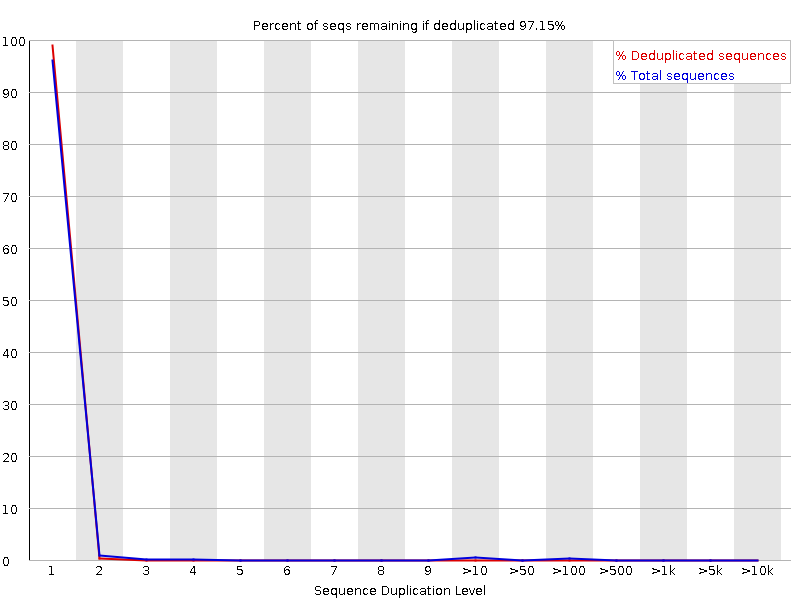
\includegraphics{/homework_02/CEBPA/duplication_levels.png}
\caption{image insertion test}
\end{figure}

\hypertarget{practical-alignment-m.musculus-cebpa-chip-seq-alignment}{%
\section{Practical: Alignment (M.Musculus CEBPA ChIP-seq
alignment)}\label{practical-alignment-m.musculus-cebpa-chip-seq-alignment}}

Cluster location of processed mouse (mm10) reference genome and index
files:

mm10 reference genome:
/mnt/Archives/genome/mouse/mm10/UCSC/bwa-0.7.15-index/index/mm10.fa

mm10 index files:
/mnt/Archives/genome/mouse/mm10/UCSC/bwa-0.7.15-index/index/mm10.fa.amb
/mnt/Archives/genome/mouse/mm10/UCSC/bwa-0.7.15-index/index/mm10.fa.ann
/mnt/Archives/genome/mouse/mm10/UCSC/bwa-0.7.15-index/index/mm10.fa.bwt
/mnt/Archives/genome/mouse/mm10/UCSC/bwa-0.7.15-index/index/mm10.fa.pac
/mnt/Archives/genome/mouse/mm10/UCSC/bwa-0.7.15-index/index/mm10.fa.sa

\begin{verbatim}
# executes fastqc for the compressed M.Musculus CEBPA (CCAAT/enhancer-binding protein alpha) transcription factor Chip-seq data file (mus_musculus_CEBPA_liver_ERR005132.fastq.gz)
fastqc /mnt/Citosina/amedina/ejorquera/BioInfoII/Tarea_2/mus_musculus_CEBPA_liver_ERR005132.fastq.gz -o output

# copies the html and compressed images output of fastqc for the CEBPA ChIP-seq data from the output folder located in the cluster into a local directory, so it can be easily opened 
# fastqc compressed images output
scp ejorquera@dna.lavis.unam.mx:/mnt/Citosina/amedina/ejorquera/BioInfoII/Tarea_2/output/mus_musculus_CEBPA_liver_ERR005132_fastqc.zip /home/esteban/Tarea_2_Results
# fastqc html report
scp ejorquera@dna.lavis.unam.mx:/mnt/Citosina/amedina/ejorquera/BioInfoII/Tarea_2/output/mus_musculus_CEBPA_liver_ERR005132_fastqc.html /home/esteban/Tarea_2_Results
\end{verbatim}

Considering the file sizes of both the mus musculus reference genome and
the CEBPA ChIP-seq data, the memory available to qlogin sessions might
not be enough, and would likely cause the process to hang indefinitely.
Therefore a sge script was generated.

\begin{verbatim}
#!/bin/bash
# Use current working directory
#$ -cwd
#
# Join stdout and stderr
#$ -j y
#
# Run job through bash shell
#$ -S /bin/bash
#
#You can edit the scriptsince this line
#
# Your job name
#$ -N Marlon_job

# Send an email after the job has finished
#$ -m e
#$ -M aldarchez26@gmail.com
#
# If modules are needed, source modules environment (Do not delete the next line):
. /etc/profile.d/modules.sh
#
# Add any modules you might require
(module load bwa/0.7.15 ; bwa mem -M -t 8 /mnt/Archives/genome/mouse/mm10/UCSC/bwa-0.7.15-index/index/mm10.fa /mnt/Timina/bioinfoII/data/alignment/mus_musculus_CEBPA_liver_ERR005132.fastq.gz > /mnt/Timina/bioinfoII/marciniega/tarea_02/MMusculus_FNR_ChIP.sam)
\end{verbatim}

\begin{verbatim}
# runs the sge script to generate the CEBPA ChIP-seq data alignment in sam file format
qsub MMusculus.sge

# uses samtools stats to save  its output to a text file
samtools stats MMusculus_FNR_ChIP.sam > MMusculus_FNR_ChIP.stats

# loads samtools stats output into the nano text editor so it can be visualized
nano  MMusculus_FNR_ChIP.stats
\end{verbatim}

\begin{figure}
\centering
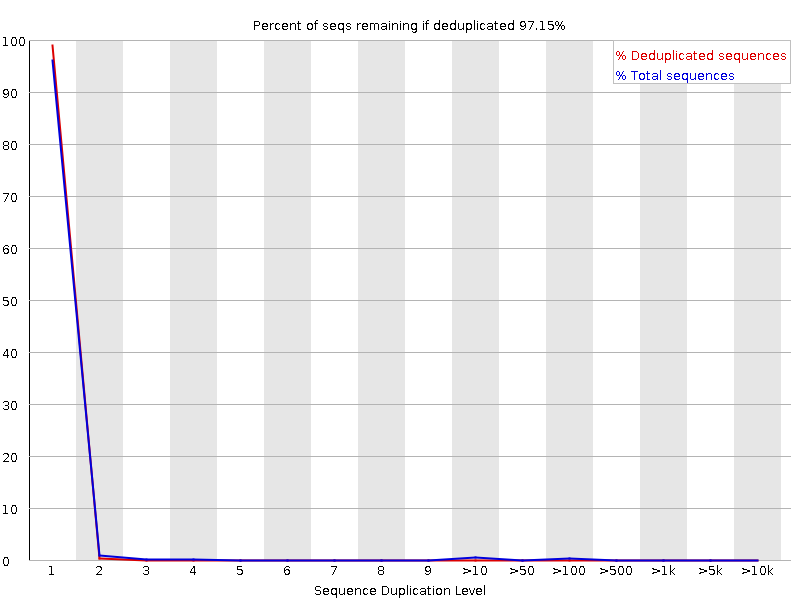
\includegraphics{/homework_02/CEBPA/duplication_levels.png}
\caption{image insertion test}
\end{figure}

\end{document}
